%  LaTeX support: latex@mdpi.com 
%  For support, please attach all files needed for compiling as well as the log file, and specify your operating system, LaTeX version, and LaTeX editor.

%=================================================================
\documentclass[journal,article,submit,pdftex,moreauthors]{Definitions/mdpi} 
%\documentclass[preprints,article,submit,pdftex,moreauthors]{Definitions/mdpi} 
% For posting an early version of this manuscript as a preprint, you may use "preprints" as the journal. Changing "submit" to "accept" before posting will remove line numbers.

% Below journals will use APA reference format:
% admsci, aieduc, behavsci, businesses, econometrics, economies, education, ejihpe, famsci, games, humans, ijcs, ijfs, jintelligence, journalmedia, jrfm, jsam, languages, peacestud, psycholint, publications, tourismhosp, youth

% Below journals will use Chicago reference format:
% arts, genealogy, histories, humanities, laws, literature, religions, risks, socsci

%--------------------
% Class Options:
%--------------------
%----------
% journal
%----------
% Choose between the following MDPI journals:
% accountaudit, acoustics, actuators, addictions, adhesives, admsci, adolescents, aerobiology, aerospace,
% agriculture, agriengineering, agrochemicals, agronomy, ai, aichem, aieduc, aieng, aimater, aimed, aipa, air,
% aisens, algorithms, allergies, alloys, amh, analog, analytica, analytics, anatomia, anesthres, animals,
% antibiotics, antibodies, antioxidants, applbiosci, appliedchem, appliedmath, appliedphys, applmech,
% applmicrobiol, applnano, applsci, aquacj, architecture, arm, arthropoda, arts, asc, asi, astronautics,
% astronomy, atmosphere, atoms, audiolres, automation, axioms, bacteria, batteries, bdcc, behavsci, beverages,
% biochem, bioengineering, biologics, biology, biomass, biomechanics, biomed, biomedicines, biomedinformatics,
% biomimetics, biomolecules, biophysica, bioresourbioprod, biosensors, biosphere, biotech, birds, blockchains,
% bloods, blsf, brainsci, breath, buildings, businesses, cancers, carbon, cardio, cardiogenetics,
% cardiovascmed, catalysts, cells, ceramics, challenges, chemengineering, chemistry, chemosensors, chemproc,
% children, chips, cimb, civileng, cleantechnol, climate, clinbioenerg, clinpract, clockssleep, cmd, cmtr,
% coasts, coatings, colloids, colorants, commodities, complexities, complications, compounds, computation,
% computers, condensedmatter, conservation, constrmater, cosmetics, covid, crops, cryo, cryptography, crystals,
% csmf, ctn, culture, curroncol, cyber, dairy, data, ddc, dentistry, dermato, dermatopathology, designs,
% devices, dhi, diabetology, diagnostics, dietetics, digital, disabilities, diseases, diversity, dna, drones,
% dynamics, earth, ebj, ecm, ecologies, econometrics, economies, edm, education, eesp, ejihpe, electricity,
% electrochem, electronicmat, electronics, encyclopedia, endocrines, energies, eng, engproc, entomology,
% entropy, environments, environremediat, epidemiologia, epigenomes, esa, est, famsci, fermentation, fibers,
% fintech, fire, fishes, fluids, foods, forecasting, forensicsci, forests, fossstud, foundations, fractalfract,
% fuels, future, futureinternet, futurepharmacol, futurephys, futuretransp, galaxies, games, gases, gastroent,
% gastrointestdisord, gastronomy, gels, genealogy, genes, geographies, geohazards, geomatics, geometry,
% geosciences, geotechnics, geriatrics, germs, glacies, grasses, green, greenhealth, gucdd, hardware,
% hazardousmatters, healthcare, hearts, hemato, hematolrep, hep, heritage, higheredu, highthroughput,
% histories, horticulturae, hospitals, humanities, humans, hydrobiology, hydrogen, hydrology, hydropower,
% hygiene, idr, iic, ijcs, ijem, ijerph, ijfs, ijgi, ijmd, ijms, ijns, ijom, ijpb, ijt, ijtm, ijtpp, ime,
% immuno, informatics, information, infrastructures, inorganics, insects, instruments, inventions, iot, j,
% jaestheticmed, jal, jcdd, jcm, jcp, jcrm, jcs, jcto, jdad, jdb, jdream, jemr, jeta, jfb, jfmk, jgbg, jgg,
% jimaging, jintelligence, jlpea, jmahp, jmmp, jmms, jmp, jmse, jne, jnt, jof, joi, joitmc, joma, jop, joptm,
% jor, journalmedia, jox, jpbi, jphytomed, jpm, jrfm, jsam, jsan, jtaer, jvd, jzbg, kidneydial,
% kinasesphosphatases, knowledge, labmed, laboratories, lae, land, languages, laws, life, lights, limnolrev,
% lipidology, liquids, literature, livers, logics, logistics, lubricants, lymphatics, machines, macromol,
% magnetism, magnetochemistry, make, marinedrugs, materials, materproc, mathematics, mca, measurements,
% medicina, medicines, medsci, membranes, merits, metabolites, metals, meteorology, methane, metrics,
% metrology, micro, microarrays, microbiolres, microelectronics, micromachines, microorganisms, microplastics,
% microwave, minerals, mining, mmphys, modelling, molbank, molecules, mps, msf, mti, multimedia, muscles,
% nanoenergyadv, nanomanufacturing, nanomaterials, ncrna, ndt, network, neuroglia, neuroimaging, neurolint,
% neurosci, nitrogen, notspecified, nursrep, nutraceuticals, nutrients, obesities, occuphealth, oceans, ohbm,
% onco, optics, oral, organics, organoids, osteology, oxygen, pandemics, parasites, parasitologia, particles,
% pathogens, pathophysiology, peacestud, pediatrrep, pets, pharmaceuticals, pharmaceutics,
% pharmacoepidemiology, pharmacy, philosophies, photochem, photonics, phycology, physchem, physics,
% physiologia, plants, plasma, platforms, pollutants, polymers, polysaccharides, populations, poultry, powders,
% precipitation, precisoncol, preprints, proceedings, processes, prosthesis, proteomes, psf, psychiatryint,
% psychoactives, psycholint, publications, purification, quantumrep, quaternary, qubs, radiation, rdt,
% reactions, realestate, receptors, recycling, regeneration, religions, remotesensing, reports, reprodmed,
% resources, rheumato, risks, rjpm, robotics, rsee, ruminants, safety, sci, scipharm, sclerosis, seeds,
% sensors, separations, sexes, shi, signals, sinusitis, siuj, skins, smartcities, sna, societies, socsci,
% software, soilsystems, solar, solids, spectroscj, sports, standards, stats, std, stratsediment, stresses,
% surfaces, surgeries, suschem, sustainability, symmetry, synbio, systems, tae, targets, taxonomy,
% technologies, telecom, test, textiles, thalassrep, therapeutics, thermo, timespace, tomography, tourismhosp,
% toxics, toxins, tph, transplantology, transportation, traumacare, traumas, tri, tropicalmed, universe,
% urbansci, uro, vaccines, vehicles, venereology, vetsci, vibration, virtualworlds, viruses, vision, waste,
% water, welding, wem, wevj, wild, wind, women, world, youth, zoonoticdis

%---------
% article
%---------
% The default type of manuscript is "article", but can be replaced by: 
% abstract, addendum, article, benchmark, book, bookreview, briefcommunication, briefreport, casereport, changes, clinicopathologicalchallenge, comment, commentary, communication, conceptpaper, conferenceproceedings, correction, conferencereport, creative, datadescriptor, discussion, entry, expressionofconcern, extendedabstract, editorial, essay, erratum, fieldguide, hypothesis, interestingimages, letter, meetingreport, monograph, newbookreceived, obituary, opinion, proceedingpaper, projectreport, reply, retraction, review, perspective, protocol, shortnote, studyprotocol, supfile, systematicreview, technicalnote, viewpoint, guidelines, registeredreport, tutorial,  giantsinurology, urologyaroundtheworld
% supfile = supplementary materials

%----------
% submit
%----------
% The class option "submit" will be changed to "accept" by the Editorial Office when the paper is accepted. This will only make changes to the frontpage (e.g., the logo of the journal will get visible), the headings, and the copyright information. Also, line numbering will be removed. Journal info and pagination for accepted papers will also be assigned by the Editorial Office.

%------------------
% moreauthors
%------------------
% If there is only one author the class option oneauthor should be used. Otherwise use the class option moreauthors.

%---------
% pdftex
%---------
% The option pdftex is for use with pdfLaTeX. Remove "pdftex" for (1) compiling with LaTeX & dvi2pdf (if eps figures are used) or for (2) compiling with XeLaTeX.

%=================================================================
% MDPI internal commands - do not modify
\firstpage{1} 
\makeatletter 
\setcounter{page}{\@firstpage} 
\makeatother
\pubvolume{1}
\issuenum{1}
\articlenumber{0}
\pubyear{2026}
\copyrightyear{2026}
%\externaleditor{Firstname Lastname} % More than 1 editor, please add `` and '' before the last editor name
\datereceived{ } 
\daterevised{ } % Comment out if no revised date
\dateaccepted{ } 
\datepublished{ } 
%\datecorrected{} % For corrected papers: "Corrected: XXX" date in the original paper.
%\dateretracted{} % For retracted papers: "Retracted: XXX" date in the original paper.
%\doinum{} % Used for some special journals, like molbank
%\pdfoutput=1 % Uncommented for upload to arXiv.org
%\CorrStatement{yes}  % For updates
%\longauthorlist{yes} % For many authors that exceed the left citation part
%\IsAssociation{yes} % For association journals

%=================================================================
% Add packages and commands here. The following packages are loaded in our class file: fontenc, inputenc, calc, indentfirst, fancyhdr, graphicx, epstopdf, lastpage, ifthen, float, amsmath, amssymb, lineno, setspace, enumitem, mathpazo, booktabs, titlesec, etoolbox, tabto, xcolor, colortbl, soul, multirow, microtype, tikz, totcount, changepage, attrib, upgreek, array, tabularx, pbox, ragged2e, tocloft, marginnote, marginfix, enotez, amsthm, natbib, hyperref, cleveref, scrextend, url, geometry, newfloat, caption, draftwatermark, seqsplit
% cleveref: load \crefname definitions after \begin{document}

% Added for the Results and Discussion section: a centered, width-flexible
% column type for the benchmark tables. Figures are external PDFs produced by
% plot_results.py (in ./figures); graphicx is already loaded by the MDPI class.
\newcolumntype{C}{>{\centering\arraybackslash}X}

%=================================================================
% Please use the following mathematics environments: Theorem, Lemma, Corollary, Proposition, Characterization, Property, Problem, Example, ExamplesandDefinitions, Hypothesis, Remark, Definition, Notation, Assumption
%% For proofs, please use the proof environment (the amsthm package is loaded by the MDPI class).

%=================================================================
% Full title of the paper (Capitalized)
\Title{Benchmarking Local Large Language Models for Structured Knowledge Extraction in Conversational Commerce}

% Author Orchid ID: enter ID or remove command
\newcommand{\orcidauthorA}{0009-0004-4210-5756} % Add \orcidA{} behind the author's name
\newcommand{\orcidauthorB}{0009-0002-1965-7822}%Luka
\newcommand{\orcidauthorC}{0000-0002-3015-1024}%Sandi
\newcommand{\orcidauthorD}{0000-0003-0323-2600}%Vedran
\newcommand{\orcidauthorE}{0000-0002-5964-245X}%Ivan

% Authors, for the paper (add full first names)
\Author{Ratomir Karlović $^{1}$\orcidA{}, Luka Sever $^{1}$\orcidB{}, Sandi Baressi Šegota $^{1}$\orcidC{}, Vedran Mrzljak$^{2}$\orcidD{} and Ivan Lorencin $^{1}$\orcidE{}}

%\longauthorlist{yes}

% MDPI internal command: Authors, for metadata in PDF
\AuthorNames{Firstname Lastname, Firstname Lastname and Firstname Lastname}

%\longauthorlist{yes}

% Affiliations / Addresses (Add [1] after \address if there is only one affiliation.)
\address{%
$^{1}$ \quad Faculty of Informatics, Juraj Dobrila University of Pula, Zagrebačka 30, 52100 Pula, Croatia;\\ ratomir.karlovic@unipu.hr (R.K.), luka.sever@unipu.hr (L.S.), sandi.baressi.segota@unipu.hr (S.B.Š.), ivan.lorencin@unipu.hr (I.L.)\\ $^{2}$ \quad Faculty of Engineering Rijeka, University of Rijeka, Vukovarska 58, 51000 Rijeka, Croatia;
}

% Contact information of the corresponding author
\corres{Correspondence: vedran.mrzljak@riteh.uniri.hr;}

% Current address and/or shared authorship
%\firstnote{Current address: Affiliation.}  
% Current address should not be the same as any items in the Affiliation section.

%\secondnote{These authors contributed equally to this work.}
% The commands \thirdnote{} till \eighthnote{} are available for further notes.

%\simplesumm{} % Simple summary

%\conference{} % An extended version of a conference paper

% Abstract (Do not insert blank lines, i.e. \\) 
\abstract{The integration of natural language understanding into conversational commerce requires robustly extracting structured intents from idiomatic text. While cloud-based models are highly capable, their latency, privacy risks, and operational costs necessitate efficient local alternatives. To address this, we empirically evaluate locally deployed, open-weights large language models (LLMs) on parsing multi-intent shopping cart commands into deterministic JSON schemas. We benchmark multiple models across minimal, extended, and few-shot prompting paradigms, utilizing a dual-axis framework to simultaneously measure extraction quality (operation F1-score, exact match, schema validity) and hardware performance (latency, GPU power consumption, VRAM usage). Our evaluation highlights a fundamental trade-off between schema compliance and computational overhead, demonstrating how advanced prompting techniques improve parsing accuracy while measurably impacting inference latency and power draw. Ultimately, this comprehensive profiling identifies optimal model configurations for resource-constrained environments, establishing a practical baseline for deploying cost-effective and energy-efficient LLMs in edge-based retail automation.}

% Keywords
\keyword{LLM; Prompt Engineering; Natural Language Understanding; JSON Parsing; Structured Output; Model Performance; Conversational Agents; Information Extraction;}

% The fields PACS, MSC, and JEL may be left empty or commented out if not applicable
%\PACS{J0101}
%\MSC{}
%\JEL{}

%%%%%%%%%%%%%%%%%%%%%%%%%%%%%%%%%%%%%%%%%%
% Only for the journal Diversity
%\LSID{\url{http://}}

%%%%%%%%%%%%%%%%%%%%%%%%%%%%%%%%%%%%%%%%%%
% Only for the journal Applied Sciences
%\featuredapplication{Authors are encouraged to provide a concise description of the specific application or a potential application of the work. This section is not mandatory.}
%%%%%%%%%%%%%%%%%%%%%%%%%%%%%%%%%%%%%%%%%%

%%%%%%%%%%%%%%%%%%%%%%%%%%%%%%%%%%%%%%%%%%
% Only for the journal Data
%\dataset{DOI number or link to the deposited data set if the data set is published separately. If the data set shall be published as a supplement to this paper, this field will be filled by the journal editors. In this case, please submit the data set as a supplement.}
%\datasetlicense{License under which the data set is made available (CC0, CC-BY, CC-BY-SA, CC-BY-NC, etc.)}

%%%%%%%%%%%%%%%%%%%%%%%%%%%%%%%%%%%%%%%%%%
% Only for the journal BioTech, Fishes, Neuroimaging and Toxins
%\keycontribution{The breakthroughs or highlights of the manuscript. Authors can write one or two sentences to describe the most important part of the paper.}

%%%%%%%%%%%%%%%%%%%%%%%%%%%%%%%%%%%%%%%%%%
% Only for the journal Encyclopedia
%\encyclopediadef{For entry manuscripts only: please provide a brief overview of the entry title instead of an abstract.}

%%%%%%%%%%%%%%%%%%%%%%%%%%%%%%%%%%%%%%%%%%
% Different journals have different requirements. Please check the specific journal guidelines in the "Instructions for Authors" on the journal's official website.
%\addhighlights{yes}
%\renewcommand{\addhighlights}{%
%
%\noindent The goal is to increase the discoverability and readability of the article via search engines and other scholars. Highlights should not be a copy of the abstract, but a simple text allowing the reader to quickly and simplified find out what the article is about and what can be cited from it. Each of these parts should be devoted up to 2~bullet points.\vspace{3pt}\\
%\textbf{What are the main findings?}
% \begin{itemize}[labelsep=2.5mm,topsep=-3pt]
% \item First bullet.
% \item Second bullet.
% \end{itemize}\vspace{3pt}
%\textbf{What are the implications of the main findings?}
% \begin{itemize}[labelsep=2.5mm,topsep=-3pt]
% \item First bullet.
% \item Second bullet.
% \end{itemize}
%}

%%%%%%%%%%%%%%%%%%%%%%%%%%%%%%%%%%%%%%%%%%
\begin{document}

%%%%%%%%%%%%%%%%%%%%%%%%%%%%%%%%%%%%%%%%%%

\section{Introduction}

The template details the sections that can be used in a manuscript. Note that the order and names of article sections may differ from the requirements of the journal (e.g., the positioning of the Materials and Methods section). Please check the instructions on the authors' page of the journal to verify the correct order and names. For any questions, please contact the editorial office of the journal or support@mdpi.com. For LaTeX-related questions please contact latex@mdpi.com.%\endnote{This is an endnote.} % To use endnotes, please un-comment \printendnotes below (before References). Only journal Laws uses \footnote.

% The order of the section titles is different for some journals. Please refer to the "Instructions for Authors” on the journal homepage.

\section{Background and Related Work}

%%%%%%%%%%%%%%%%%%%%%%%%%%%%%%%%%%%%%%%%%%
\section{Methodology}

Materials and Methods should be described with sufficient details to allow others to replicate and build on published results. Please note that publication of your manuscript implicates that you must make all materials, data, computer code, and protocols associated with the publication available to readers. Please disclose at the submission stage any restrictions on the availability of materials or information. New methods and protocols should be described in detail while well-established methods can be briefly described and appropriately cited.

Research manuscripts reporting large datasets that are deposited in a publicly avail-able database should specify where the data have been deposited and provide the relevant accession numbers. If the accession numbers have not yet been obtained at the time of submission, please state that they will be provided during review. They must be provided prior to publication.

Interventionary studies involving animals or humans, and other studies require ethical approval must list the authority that provided approval and the corresponding ethical approval code.

In this section, where applicable, authors are required to disclose details of how gen-erative artificial intelligence (GenAI) has been used in this paper (e.g., to generate text, data, or graphics, or to assist in study design, data collection, analysis, or interpretation). The use of GenAI for superficial text editing (e.g., grammar, spelling, punctuation, and formatting) does not need to be declared.

%%%%%%%%%%%%%%%%%%%%%%%%%%%%%%%%%%%%%%%%%%
\section{Results and Discussion}

We evaluate six open-weights models under three prompting regimes---\emph{minimal}, \emph{extended}, and \emph{few-shot}---yielding 18 model--prompt configurations, each applied to the full set of 5000 held-out shopping-cart commands. These commands contain a mean of 3.64 atomic operations (18{,}175 gold operations in total), so a single utterance typically bundles several add/remove intents that must be jointly recovered. Following the dual-axis protocol introduced in the Methodology, we report extraction quality (Table~\ref{tab:quality}) and computational cost (Table~\ref{tab:cost}) for every configuration, and then analyse the quality--cost trade-off that the prompting regime induces (Figure~\ref{fig:tradeoff}). Throughout, we use the operation-level micro-averaged F1 score (Op-F1) as the primary quality scalar and an estimated energy per command, $E \approx \bar{P}\,\bar{t}$ (mean GPU power $\times$ mean latency), as the primary cost scalar.

\subsection{Extraction Quality and the Role of the Prompting Regime}

\begin{table}[H]
\caption{Extraction quality by model and prompting regime (Min, minimal; Ext, extended; FS, few-shot). JSON and Schema denote the JSON- and schema-validity rates; Op-F1 is the operation-level micro-averaged F1 score; EM is the ordered full-command exact-match rate; Act, Prod, and Qty are the action-, product-, and quantity-field accuracies. All values are computed over the 5000-command evaluation set. The best Op-F1 per model is shown in bold.\label{tab:quality}}
\footnotesize
\begin{tabularx}{\textwidth}{l l *{7}{C}}
\toprule
\textbf{Model} & \textbf{Prompt} & \textbf{JSON} & \textbf{Schema} & \textbf{Op-F1} & \textbf{EM} & \textbf{Act} & \textbf{Prod} & \textbf{Qty} \\
\midrule
\multirow{3}{*}{Gemma4 31B} & Min & 1.000 & 1.000 & 0.951 & 0.833 & 0.969 & 0.995 & 0.984 \\
 & Ext & 1.000 & 1.000 & 0.967 & 0.885 & 0.978 & 1.000 & 0.989 \\
 & FS & 1.000 & 1.000 & \textbf{0.981} & 0.933 & 0.981 & 1.000 & 1.000 \\
\midrule
\multirow{3}{*}{GPT-OSS 20B} & Min & 1.000 & 1.000 & 0.923 & 0.753 & 0.968 & 0.991 & 0.958 \\
 & Ext & 0.999 & 0.999 & 0.944 & 0.819 & 0.981 & 0.994 & 0.967 \\
 & FS & 1.000 & 1.000 & \textbf{0.975} & 0.915 & 0.995 & 0.999 & 0.980 \\
\midrule
\multirow{3}{*}{Llama3.1 8B} & Min & 0.935 & 0.881 & 0.782 & 0.538 & 0.856 & 0.808 & 0.853 \\
 & Ext & 0.998 & 0.976 & 0.801 & 0.568 & 0.929 & 0.860 & 0.949 \\
 & FS & 0.997 & 0.995 & \textbf{0.950} & 0.841 & 0.977 & 0.966 & 0.988 \\
\midrule
\multirow{3}{*}{Mistral 7B} & Min & 0.963 & 0.877 & 0.689 & 0.357 & 0.842 & 0.762 & 0.855 \\
 & Ext & 0.982 & 0.865 & 0.504 & 0.281 & 0.871 & 0.559 & 0.887 \\
 & FS & 0.993 & 0.976 & \textbf{0.942} & 0.804 & 0.950 & 0.963 & 0.973 \\
\midrule
\multirow{3}{*}{Granite4 3B} & Min & 1.000 & 0.928 & 0.797 & 0.512 & 0.930 & 0.871 & 0.930 \\
 & Ext & 1.000 & 0.931 & 0.790 & 0.516 & 0.921 & 0.859 & 0.946 \\
 & FS & 1.000 & 0.997 & \textbf{0.937} & 0.807 & 0.984 & 0.958 & 0.987 \\
\midrule
\multirow{3}{*}{Llama3.2 3B} & Min & 0.967 & 0.606 & 0.610 & 0.311 & 0.758 & 0.700 & 0.749 \\
 & Ext & 0.970 & 0.637 & 0.526 & 0.229 & 0.681 & 0.581 & 0.754 \\
 & FS & 0.890 & 0.822 & \textbf{0.813} & 0.566 & 0.796 & 0.810 & 0.826 \\
\bottomrule
\end{tabularx}
\end{table}

Few-shot prompting yields the best Op-F1 for all six models, and the magnitude of the gain is inversely related to the model's zero-shot capability. Relative to the minimal prompt, in-context demonstrations raise Op-F1 by only $+0.031$ for Gemma4 31B and $+0.051$ for GPT-OSS 20B, but by $+0.140$ (Granite4 3B), $+0.168$ (Llama3.1 8B), $+0.203$ (Llama3.2 3B), and $+0.253$ (Mistral 7B) for the smaller models. The exemplars thus act as a capability equaliser: models that are mediocre zero-shot parsers become competitive once shown the target format, whereas the largest models---already near ceiling---have little headroom to gain. Figure~\ref{fig:f1bars} visualises this compression of the quality gap between small and large models.

\begin{figure}[H]
\centering
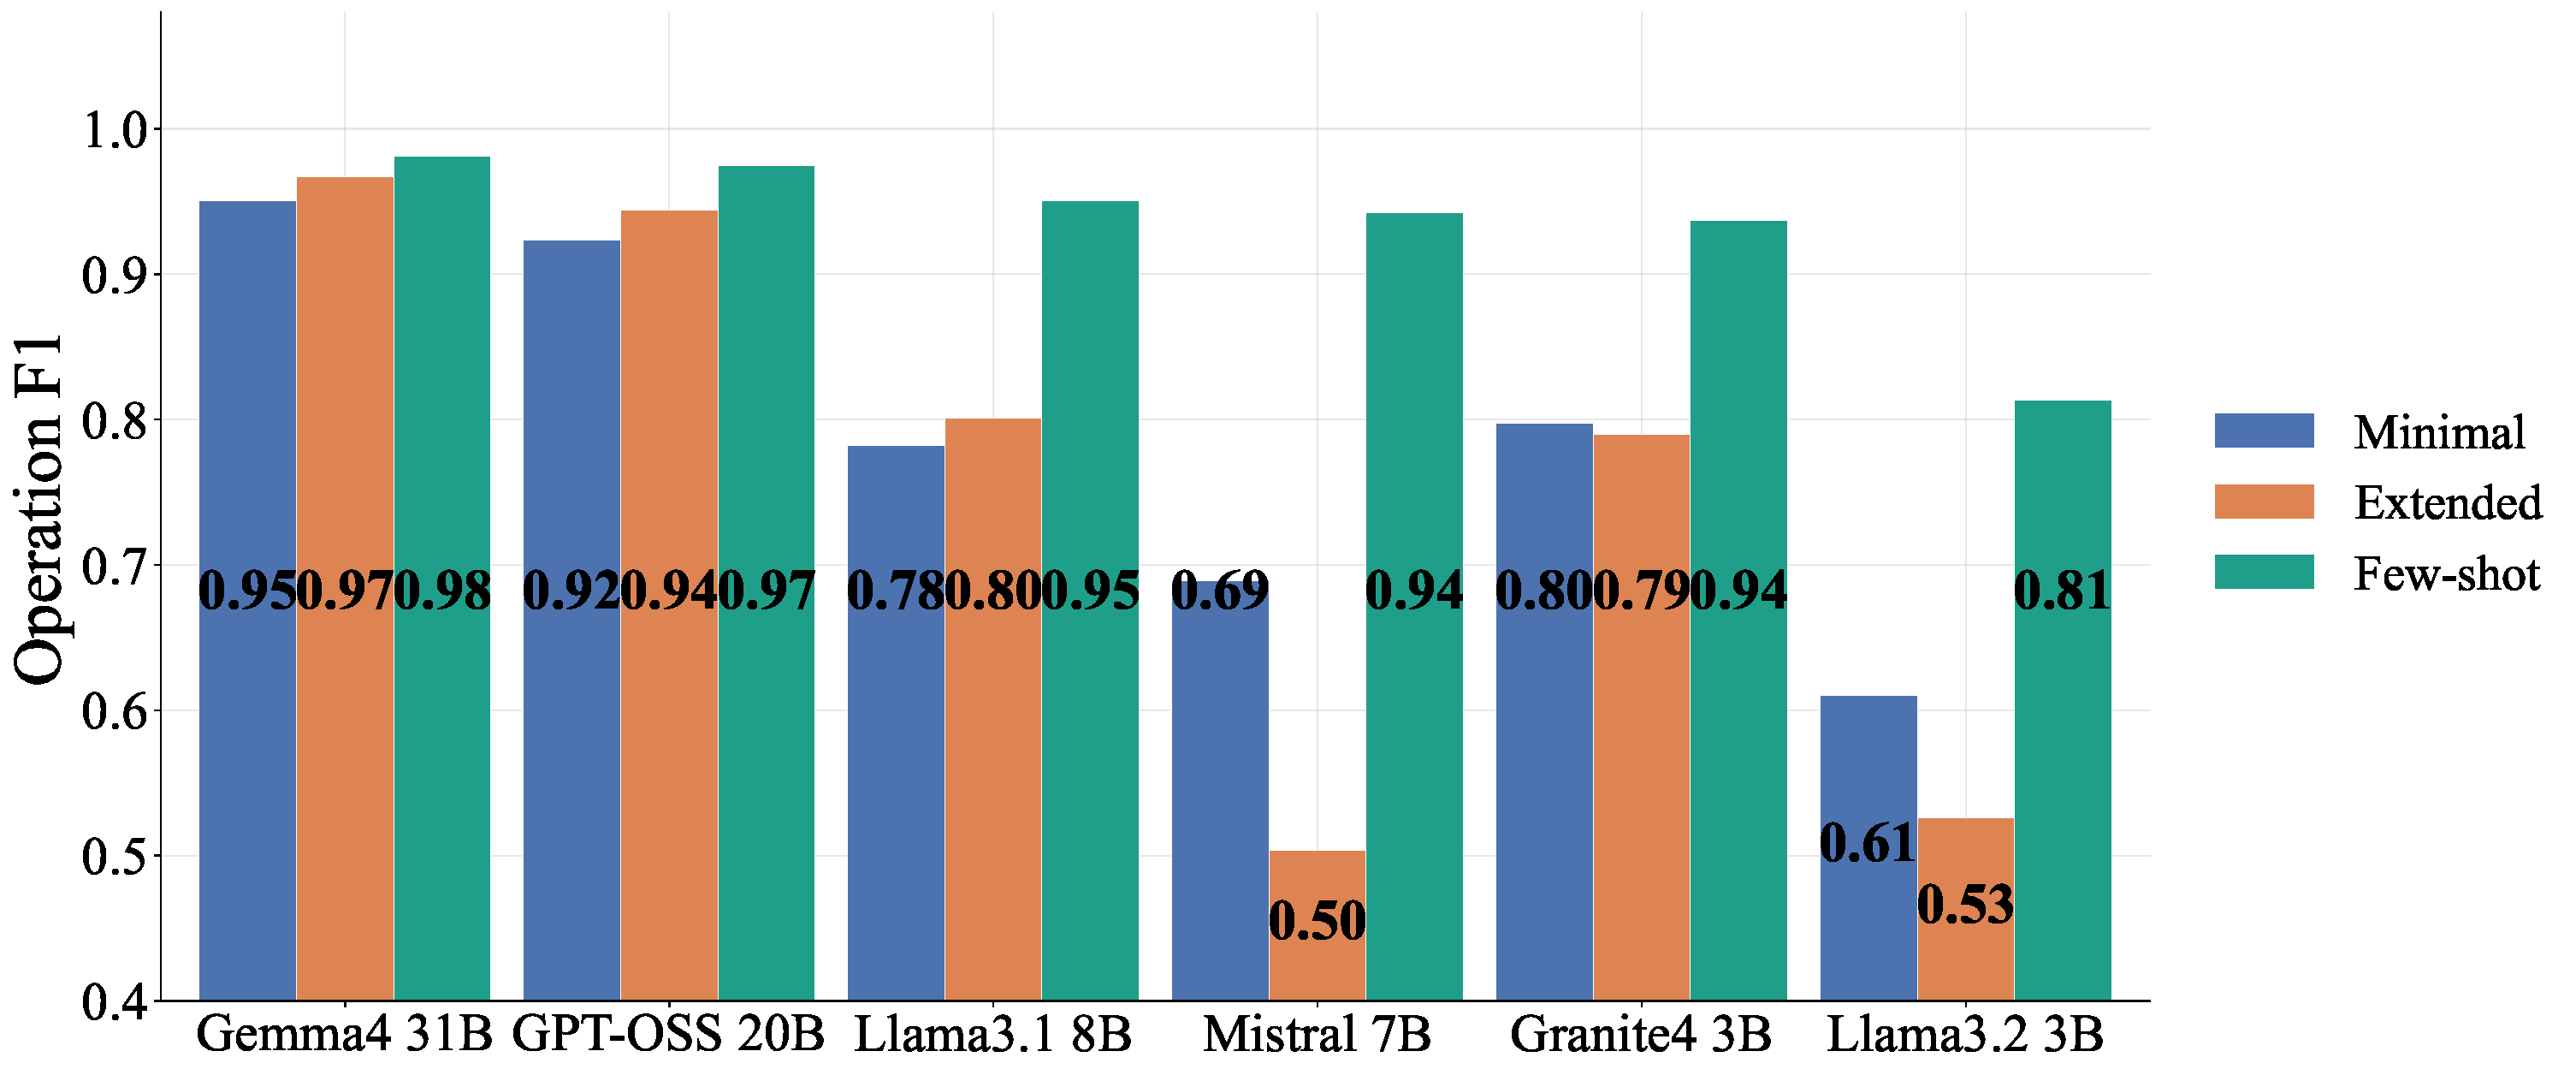
\includegraphics[width=0.8\linewidth]{figures/f1_by_regime.pdf}
\caption{Operation-level F1 by model and prompting regime. Few-shot prompting (teal) yields the best accuracy for all six models and sharply compresses the gap between small and large models; the extended prompt (orange) is inconsistent, degrading Mistral 7B and the Llama3.2 3B small model relative to the minimal prompt (blue).\label{fig:f1bars}}
\end{figure}

Decomposing quality into format adherence and content correctness clarifies the mechanism. Under the minimal prompt, several small models emit syntactically valid JSON that nonetheless violates the target schema: schema validity is only 0.928 (Granite4 3B), 0.881 (Llama3.1 8B), and 0.606 (Llama3.2 3B) despite JSON validity at or above 0.94. Few-shot demonstrations repair this format gap almost entirely---schema validity rises to 0.997, 0.995, and 0.822, respectively---indicating that the dominant failure mode of small models is structural (key naming, value typing, nesting) rather than semantic. Demonstrations specify the output contract by example rather than by description, which the smaller models follow more reliably than prose instructions. Figure~\ref{fig:qualgrid} reports all seven quality metrics across models and regimes, making this format-versus-content decomposition visually explicit.

\begin{figure}[H]
\centering
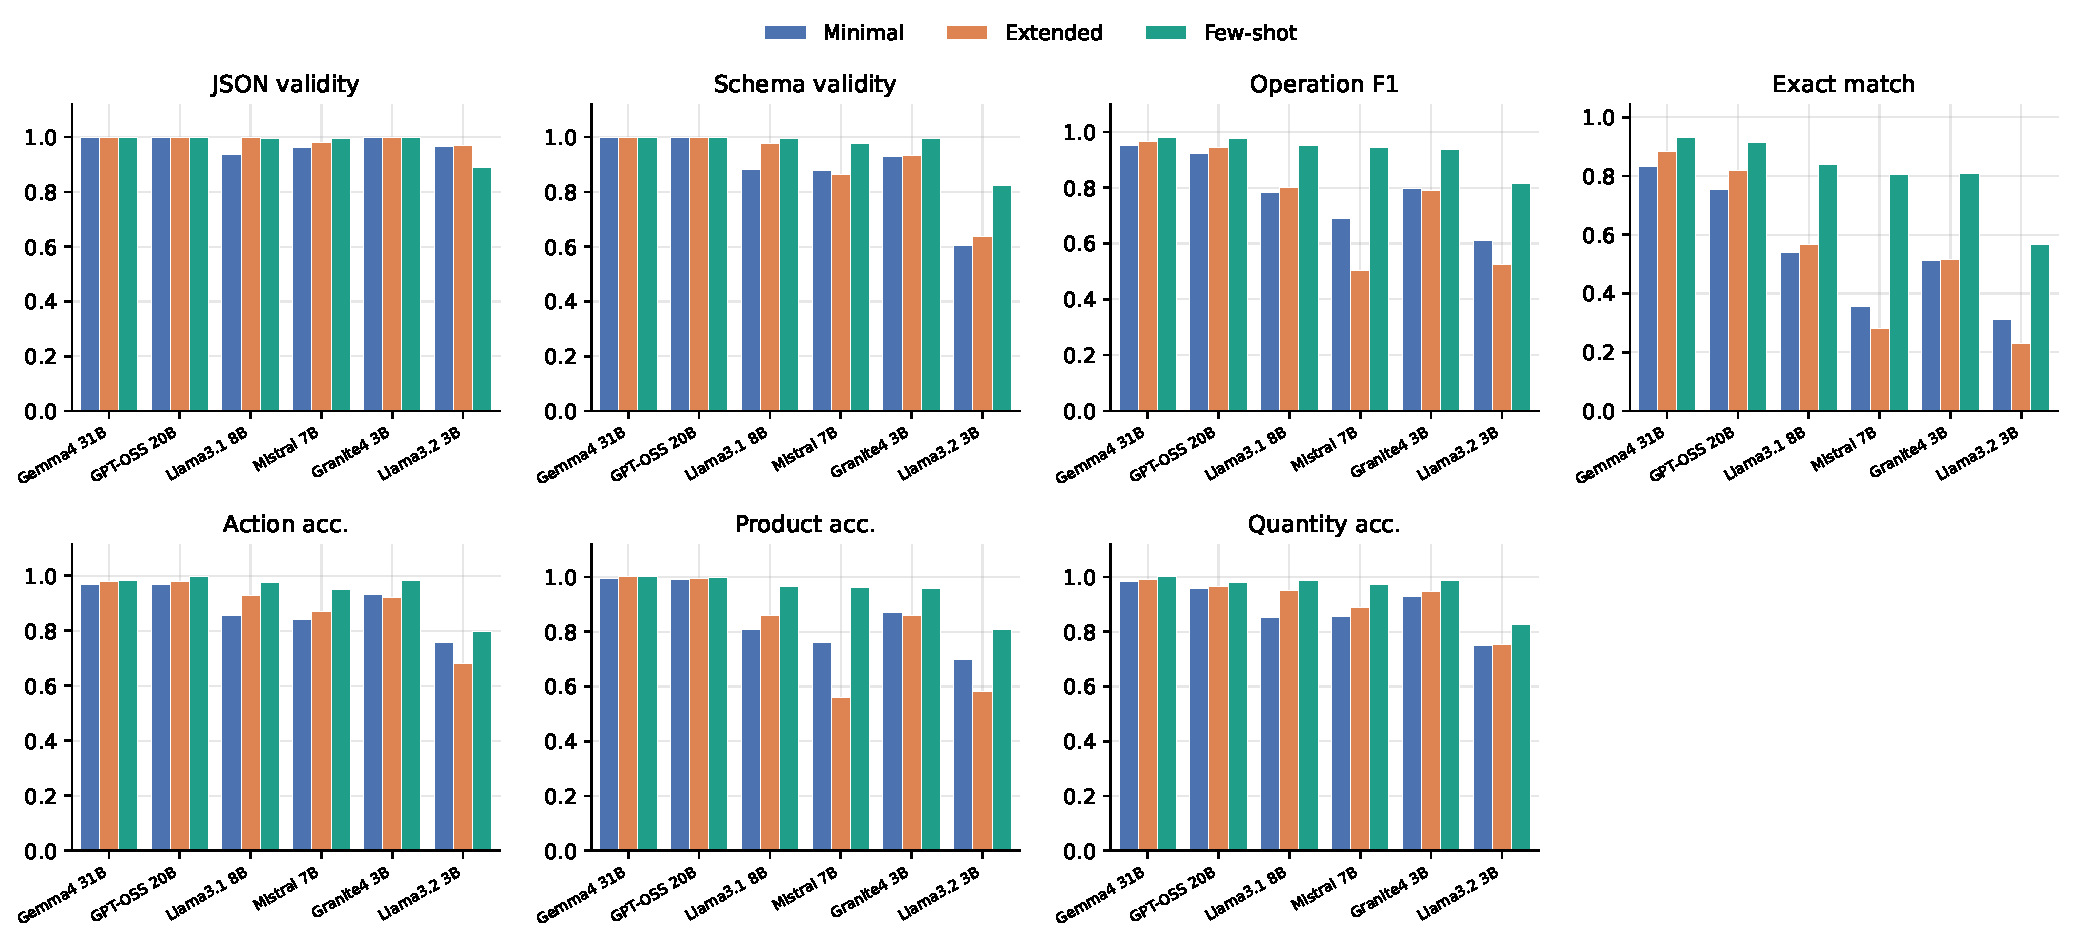
\includegraphics[width=\linewidth]{figures/quality_metrics_grid.pdf}
\caption{All quality metrics by model and prompting regime; each panel is a grouped bar chart over the six models (bars: minimal, extended, few-shot). Few-shot prompting (teal) is best across essentially every metric for the capable models, and the largest small-model gains appear on schema validity and exact match, confirming that the principal failure mode under weaker prompts is structural rather than semantic.\label{fig:qualgrid}}
\end{figure}

In contrast, the extended (instruction-rich) prompt is not a monotonic improvement and is frequently harmful. It helps only the most capable models---Gemma4 31B ($+0.016$), GPT-OSS 20B ($+0.021$), and Llama3.1 8B ($+0.019$)---while degrading Mistral 7B ($-0.185$) and Llama3.2 3B ($-0.084$), and leaving Granite4 3B essentially unchanged ($-0.007$). Manual inspection traces the Mistral regression to over-normalisation: the additional instructions induce the model to lemmatise product spans (``toothpastes'' $\rightarrow$ ``toothpaste'', ``quinoa bags'' $\rightarrow$ ``quinoa bag'') and to misresolve idiomatic quantities (``a pair'' $\rightarrow$ 1), collapsing product-field accuracy from 0.762 to 0.559 even though the emitted JSON remains well-formed. Longer instructions therefore introduce degrees of freedom that smaller models resolve in unintended, ostensibly ``helpful'' ways that diverge from the verbatim-span ground truth. This is an important negative result: scaling prompt complexity without grounding it in exemplars can reduce extraction fidelity.

\subsection{Computational Cost and the Decode-Bound Regime}

\begin{table}[H]
\caption{Computational cost by model and prompting regime. Lat$_{\mathrm{med}}$, Lat$_{\mathrm{mean}}$, and Lat$_{\mathrm{p95}}$ are latency percentiles (s); Thr is throughput (commands/s); Pwr is mean GPU power (W); $E$ is the estimated energy per command (J, $E \approx \bar{P}\,\bar{t}$); P-tok and E-tok are the mean prompt- and output-token counts. Lower is better for all columns except throughput.\label{tab:cost}}
\footnotesize
\setlength{\tabcolsep}{4pt}
\begin{tabularx}{\textwidth}{l l *{8}{C}}
\toprule
\textbf{Model} & \textbf{Prompt} & \textbf{Lat$_{\mathrm{med}}$} & \textbf{Lat$_{\mathrm{mean}}$} & \textbf{Lat$_{\mathrm{p95}}$} & \textbf{Thr} & \textbf{Pwr} & \textbf{$E$ (J)} & \textbf{P-tok} & \textbf{E-tok} \\
\midrule
\multirow{3}{*}{Gemma4 31B} & Min & 13.03 & 16.33 & 37.24 & 0.06 & 156 & 2555 & 146 & 600 \\
 & Ext & 13.25 & 16.27 & 36.62 & 0.06 & 156 & 2545 & 197 & 599 \\
 & FS & 10.10 & 11.71 & 19.87 & 0.08 & 156 & 1820 & 436 & 426 \\
\midrule
\multirow{3}{*}{GPT-OSS 20B} & Min & 2.46 & 2.54 & 3.90 & 0.36 & 124 & 315 & 196 & 345 \\
 & Ext & 2.44 & 2.52 & 3.95 & 0.36 & 124 & 313 & 248 & 341 \\
 & FS & 2.39 & 2.51 & 3.89 & 0.37 & 126 & 315 & 455 & 339 \\
\midrule
\multirow{3}{*}{Llama3.1 8B} & Min & 0.72 & 0.71 & 0.98 & 1.06 & 141 & 101 & 138 & 79 \\
 & Ext & 0.64 & 0.66 & 0.93 & 1.12 & 141 & 94 & 191 & 72 \\
 & FS & 0.58 & 0.56 & 0.71 & 1.26 & 140 & 79 & 402 & 57 \\
\midrule
\multirow{3}{*}{Mistral 7B} & Min & 0.61 & 0.59 & 0.84 & 1.24 & 146 & 87 & 148 & 88 \\
 & Ext & 0.58 & 0.56 & 0.78 & 1.30 & 147 & 82 & 200 & 82 \\
 & FS & 0.50 & 0.49 & 0.64 & 1.42 & 143 & 70 & 467 & 70 \\
\midrule
\multirow{3}{*}{Granite4 3B} & Min & 0.65 & 0.61 & 0.82 & 1.21 & 119 & 73 & 136 & 98 \\
 & Ext & 0.53 & 0.52 & 0.81 & 1.35 & 118 & 62 & 189 & 81 \\
 & FS & 0.41 & 0.39 & 0.51 & 1.64 & 118 & 46 & 400 & 56 \\
\midrule
\multirow{3}{*}{Llama3.2 3B} & Min & 0.51 & 0.53 & 0.76 & 1.34 & 123 & 65 & 148 & 90 \\
 & Ext & 0.50 & 0.49 & 0.63 & 1.42 & 124 & 61 & 201 & 80 \\
 & FS & 0.40 & 0.39 & 0.48 & 1.67 & 122 & 47 & 412 & 56 \\
\bottomrule
\end{tabularx}
\end{table}

The cost profile is governed by decoding rather than prefill. Although few-shot prompts are three- to fourfold longer on the input side (prompt tokens rise from ${\sim}140$ to ${\sim}400$--$470$), they consistently reduce wall-clock latency because the demonstrations suppress verbose generation: mean output length falls (e.g., 98 $\rightarrow$ 56 eval tokens for Granite4 3B and 600 $\rightarrow$ 426 for Gemma4 31B), and decode dominates latency in autoregressive inference. Consequently, few-shot mean latency is 17.7--35.6\% lower than minimal for five of the six models (Granite4 3B $-35.6$\%, Gemma4 31B $-28.3$\%, Llama3.2 3B $-27.2$\%, Llama3.1 8B $-21.2$\%, Mistral 7B $-17.7$\%), with GPT-OSS 20B effectively flat ($-1.4$\%). The conventional intuition that richer prompts cost more compute is thus inverted here: by constraining the output, exemplars make inference simultaneously more accurate and faster. Figure~\ref{fig:tokens} contrasts the prompt and output token counts that drive this effect.

\begin{figure}[H]
\centering
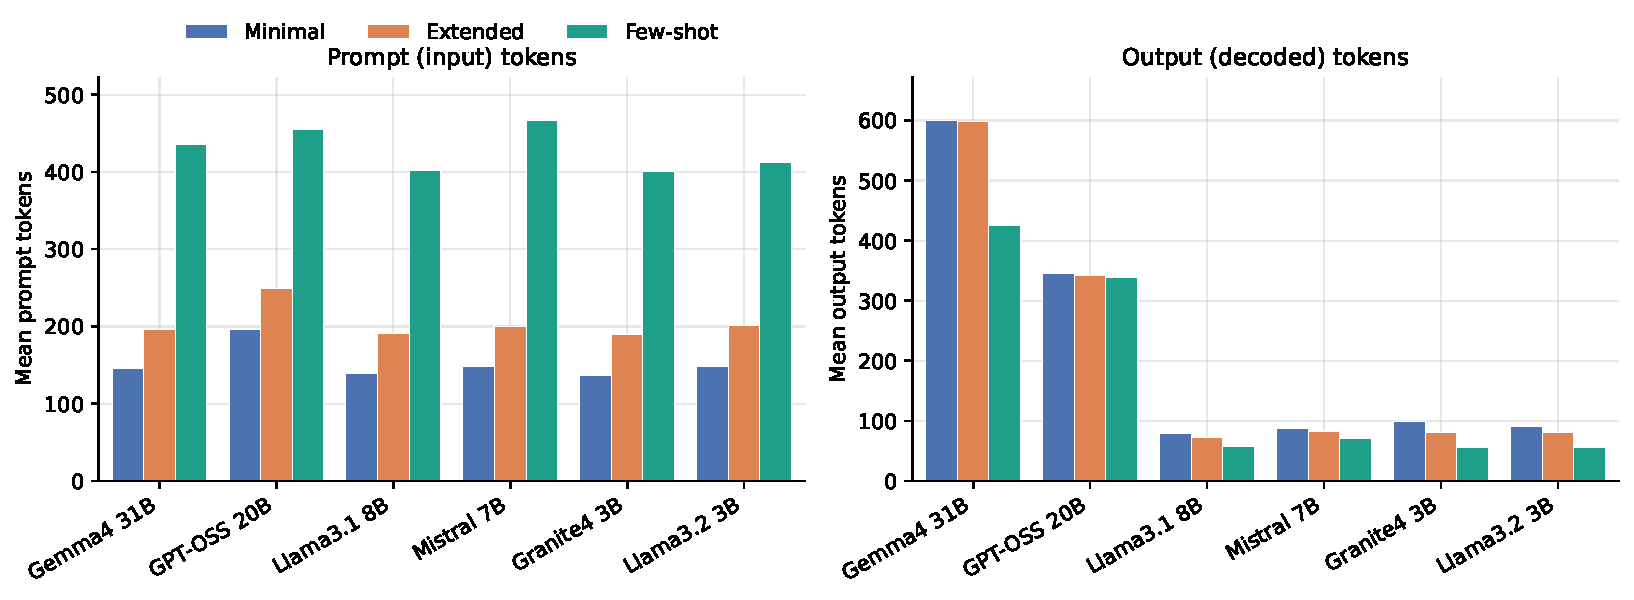
\includegraphics[width=\linewidth]{figures/tokens_by_regime.pdf}
\caption{Mean prompt (input) and output (decoded) token counts per command, by model and prompting regime. Few-shot prompts are markedly longer on the input side (left) yet \emph{shorter} on the output side (right): the demonstrations elicit concise, minified JSON and suppress verbose generation. Because decoding dominates latency, this reduction in output tokens is the mechanism behind the lower few-shot latency and energy reported in Table~\ref{tab:cost}.\label{fig:tokens}}
\end{figure}

GPU power draw is essentially model-bound rather than prompt-bound---within each model it varies by only a few watts across regimes (e.g., ${\sim}156$~W for Gemma4 31B, ${\sim}124$~W for GPT-OSS 20B, ${\sim}118$~W for Granite4 3B)---so the estimated energy per command tracks latency. Few-shot prompting therefore reduces per-command energy by 19--36\% for the capable models, with the smallest models reaching 46~J (Granite4 3B) and 47~J (Llama3.2 3B) per command versus 315~J (GPT-OSS 20B) and 1820~J (Gemma4 31B). Energy spans a factor of roughly 40 across the frontier---a far wider dynamic range than quality---which is the crux of the deployment trade-off analysed in Section~\ref{sec:tradeoff}. Figure~\ref{fig:costgrid} summarises all eight cost metrics across the 18 configurations.

We report mean VRAM occupancy in the underlying logs for completeness but caution against ranking models by it: the measured footprint does not track parameter count (the 20B GPT-OSS model occupies only ${\sim}16$~GB, less than the 3B Llama3.2 at ${\sim}17$~GB or the 8B Llama3.1 at ${\sim}22$~GB), which indicates that the figure reflects server-level allocator reservation and key--value-cache pre-allocation under the serving runtime rather than the minimal model footprint. Absolute VRAM values should accordingly be read as an upper bound on residency for this deployment, not as an intrinsic model property.

\begin{figure}[H]
\centering
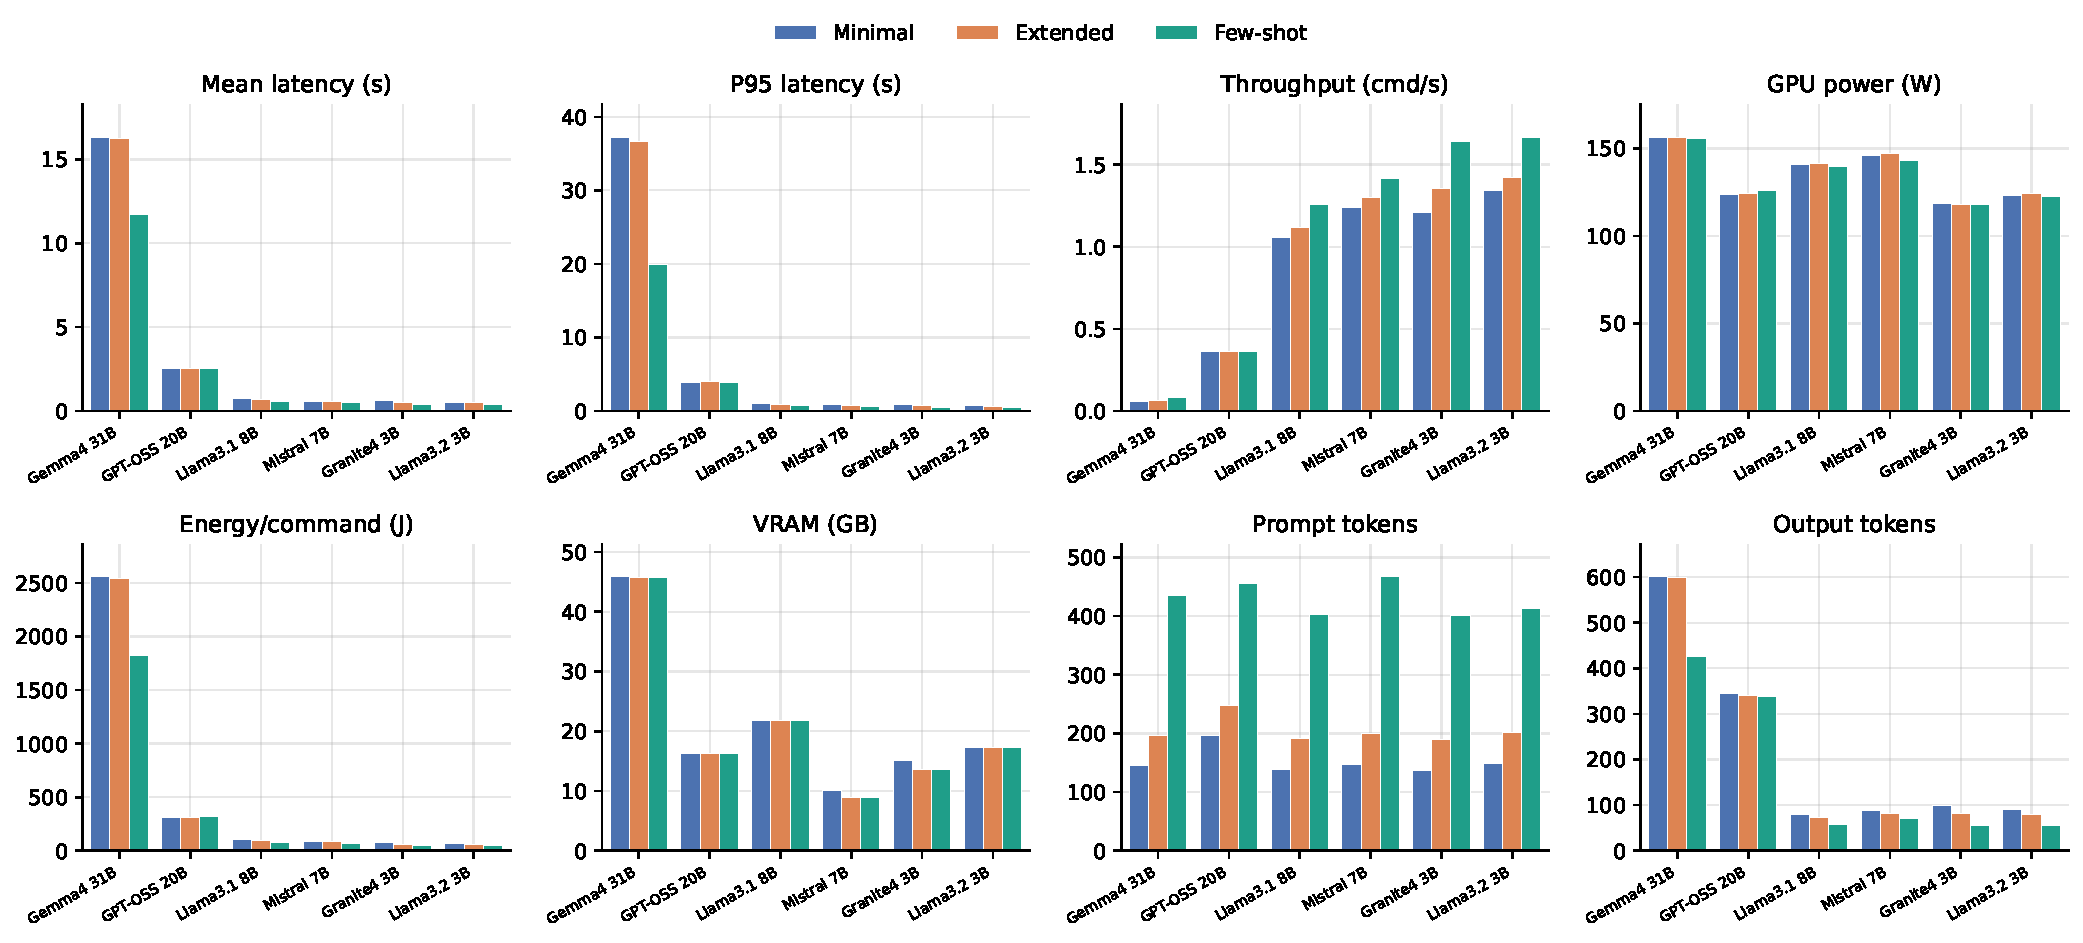
\includegraphics[width=\linewidth]{figures/cost_metrics_grid.pdf}
\caption{All cost metrics by model and prompting regime: mean and p95 latency, throughput, mean GPU power, estimated energy per command, VRAM occupancy, and mean prompt and output token counts. Latency, energy, and throughput improve under few-shot prompting for every model, whereas GPU power is essentially model-bound. The latency and energy panels are dominated by Gemma4 31B, reflecting the ${\sim}40\times$ cost dynamic range across the frontier. VRAM reflects serving-runtime reservation rather than the minimal model footprint (see text).\label{fig:costgrid}}
\end{figure}

\subsection{The Quality--Cost Trade-off}\label{sec:tradeoff}

\begin{figure}[H]
\centering
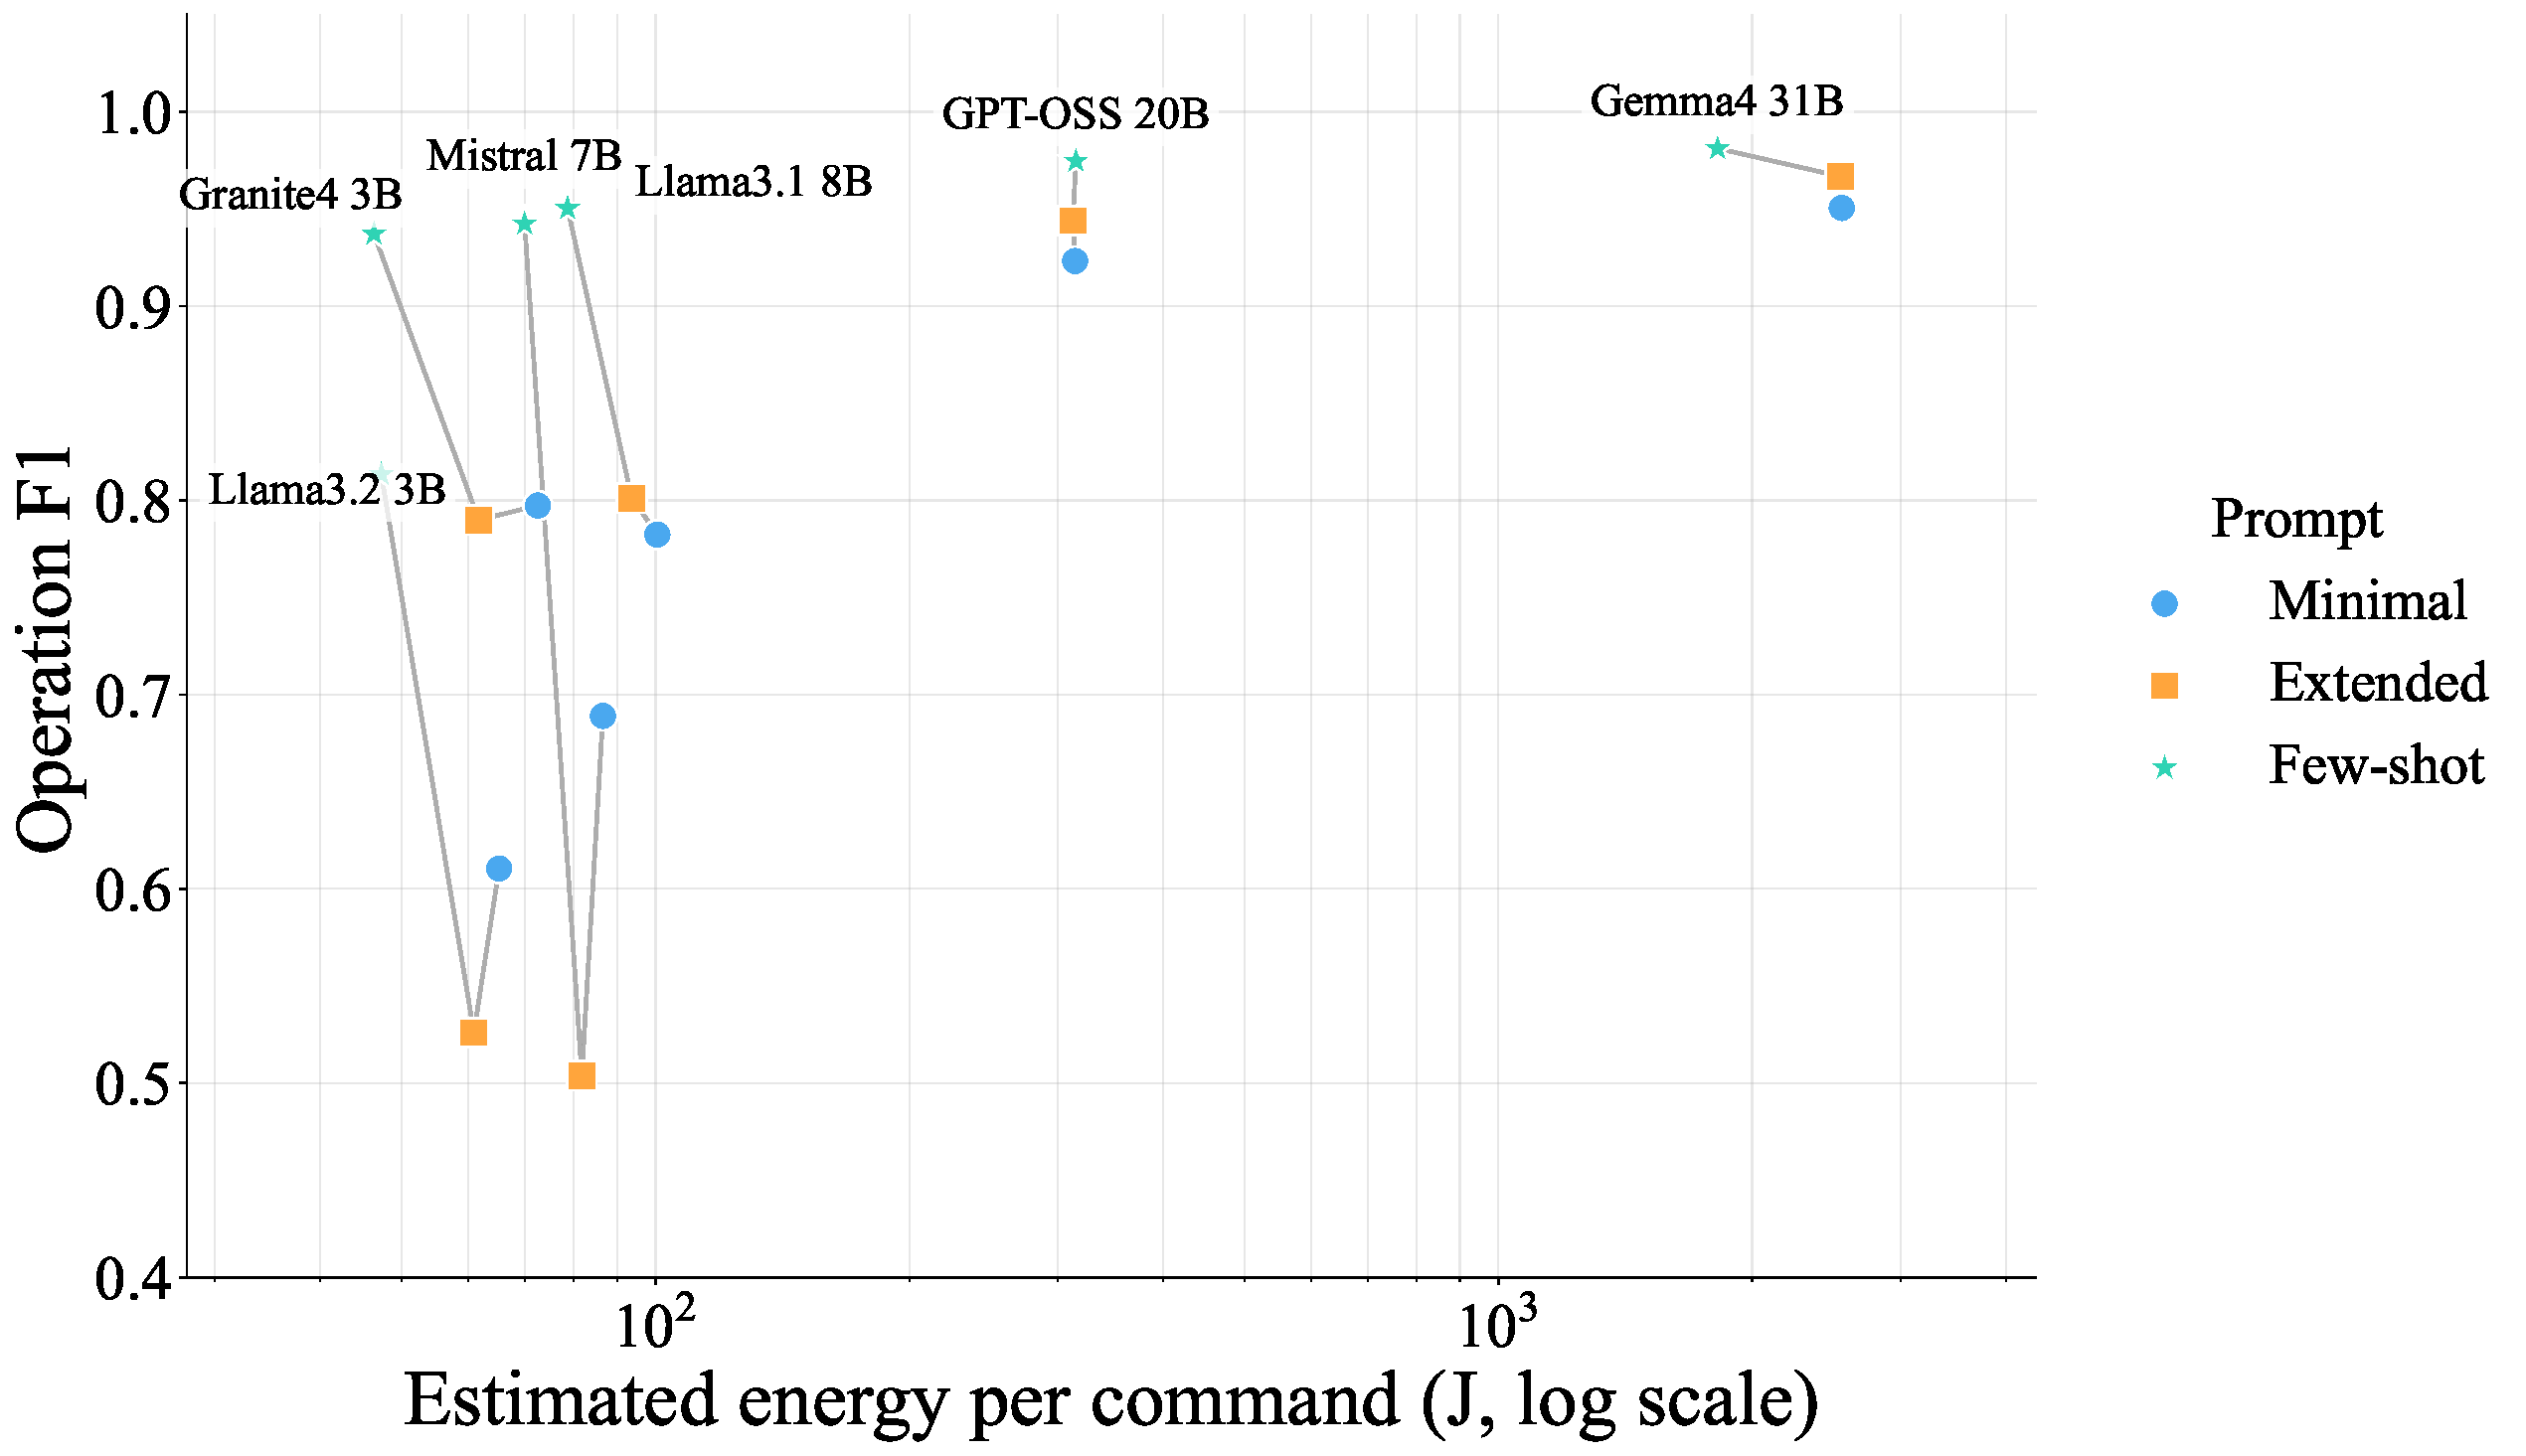
\includegraphics[width=0.88\linewidth]{figures/quality_cost_tradeoff.pdf}
\caption{Quality--cost trade-off across all 18 configurations. Each point is one model--prompt configuration; thin grey lines connect the three regimes of a model. The horizontal axis is the estimated energy per command on a logarithmic scale. For every model the few-shot configuration (star) lies above and to the left of its minimal (circle) and extended (square) counterparts---simultaneously more accurate and more energy-efficient---so the operative trade-off is across model scale along the few-shot frontier rather than across prompts.\label{fig:tradeoff}}
\end{figure}

Figure~\ref{fig:tradeoff} plots every configuration in the energy--quality plane and reveals the central finding of this study: for capable models, few-shot prompting is Pareto-improving rather than Pareto-trading---it moves each model up (higher F1) and to the left (lower energy) at once. The few-shot points dominate their own minimal and extended counterparts for all six models. The genuine trade-off is therefore not between prompts but across model scale: along the few-shot frontier, quality and cost are positively coupled, and the practitioner's decision reduces to selecting an operating point on that frontier. Three operating points are practically distinct:

\begin{itemize}[leftmargin=*,topsep=2pt,itemsep=2pt]
\item \textbf{Maximum accuracy.} Gemma4 31B (few-shot) attains the highest fidelity (Op-F1 0.981, exact match 0.933) but at 1820~J and 11.7~s per command---appropriate only where accuracy is paramount and latency and energy are unconstrained, such as offline or server-side processing.
\item \textbf{Balanced.} GPT-OSS 20B (few-shot) reaches Op-F1 0.975 at 315~J and 2.5~s, a 5.8$\times$ energy reduction for a 0.6-point F1 loss relative to Gemma4 31B.
\item \textbf{Efficiency frontier.} Granite4 3B (few-shot) achieves Op-F1 0.937---95.5\% of Gemma4 31B's quality---at 46~J and 0.39~s, that is, roughly 40$\times$ less energy and 30$\times$ lower latency. Llama3.1 8B (0.950, 79~J) and Mistral 7B (0.942, 70~J) offer marginally higher accuracy at modestly higher cost.
\end{itemize}

Quality saturates rapidly with scale once few-shot prompting is applied: moving from a 3B to a 31B model improves Op-F1 by only ${\sim}0.044$ while increasing energy by a factor of roughly 40. For the resource-constrained, edge-oriented retail setting that motivates this work, a 3--8B model with few-shot prompting is therefore the rational default, reserving 20--31B models for accuracy-critical or server-side deployments. Crucially, this recommendation is contingent on the prompt: the same small models are not viable under minimal or extended prompting (Op-F1 0.50--0.80), so the deployment win arises from the prompt--model pairing rather than from the model alone. The same Pareto structure holds when mean latency replaces energy on the cost axis (Figure~\ref{fig:lattradeoff}), confirming that the ranking of configurations is robust to the choice of cost metric.

\begin{figure}[H]
\centering
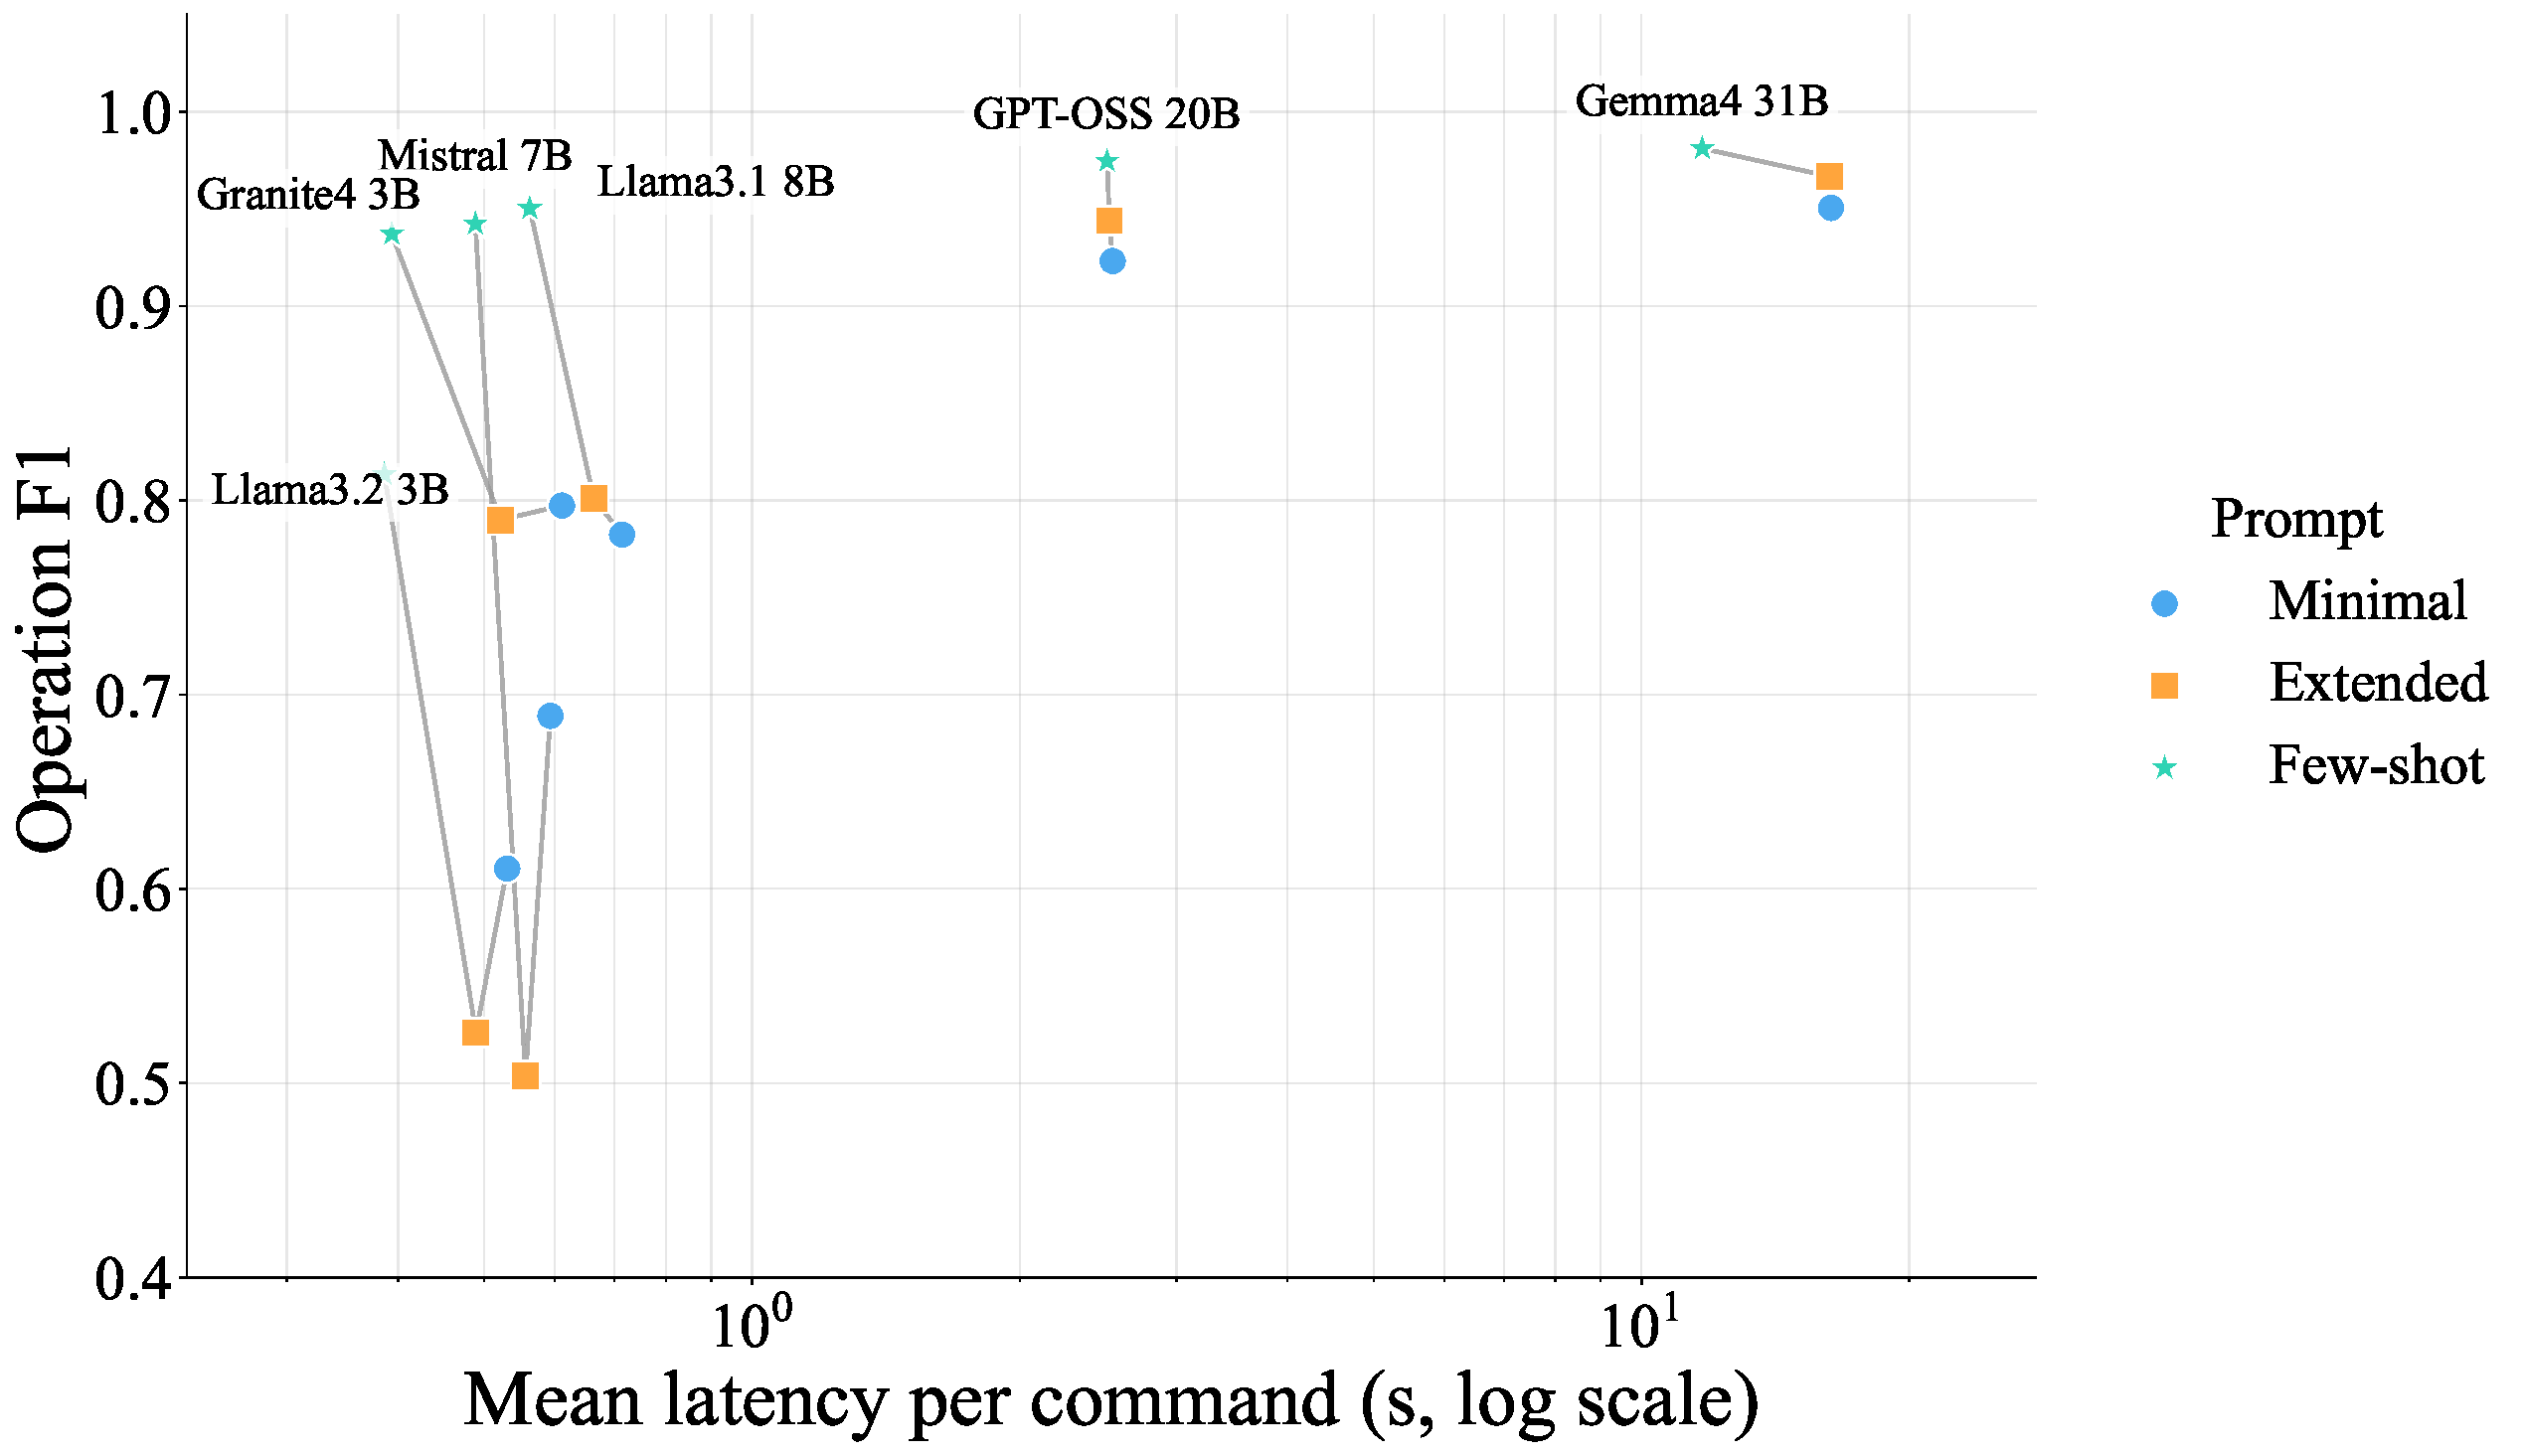
\includegraphics[width=0.88\linewidth]{figures/latency_f1_tradeoff.pdf}
\caption{Quality--cost trade-off with mean latency per command (log scale) as the cost axis, complementing Figure~\ref{fig:tradeoff}. Markers denote the prompting regime and thin lines connect the three regimes of each model. The few-shot frontier again lies up and to the left and the model ordering is preserved, confirming that the conclusions are robust to whether cost is measured as latency or energy.\label{fig:lattradeoff}}
\end{figure}

\subsection{Error Analysis}

Field-level accuracies localise the residual errors. Product-span extraction is the hardest field for every model that makes appreciable errors: under the minimal prompt the 3--8B models score only 0.70--0.87 on the product field, below both their action (0.76--0.93) and quantity (0.75--0.93) accuracies, reflecting sensitivity to surface form such as pluralisation; quantity resolution is additionally stressed by idiomatic numerals (``a pair'', ``half a dozen'', ``a dozen'') that must be mapped to integers. For the near-ceiling large models the three fields all exceed 0.95 and their differences are negligible. The gap between operation-level F1 and whole-command exact match is informative: even Gemma4 31B (few-shot) scores 0.981 Op-F1 but 0.933 exact match, because a command counts as correct only if all of its 3.64 operations on average are simultaneously correct, so per-operation errors compound multiplicatively at the command level. Exact match is consequently the more stringent and deployment-relevant metric for transactional settings, where a single misparsed item corrupts the entire cart update.

%%%%%%%%%%%%%%%%%%%%%%%%%%%%%%%%%%%%%%%%%%
\section{Limitations and Future Work}


%%%%%%%%%%%%%%%%%%%%%%%%%%%%%%%%%%%%%%%%%%
\section{Conclusions}

This section is not mandatory, but can be added to the manuscript if the discussion is unusually long or complex.

%%%%%%%%%%%%%%%%%%%%%%%%%%%%%%%%%%%%%%%%%%
\vspace{6pt} 


%%%%%%%%%%%%%%%%%%%%%%%%%%%%%%%%%%%%%%%%%%
%% optional
%\supplementary{The following supporting information can be downloaded at:  \linksupplementary{s1}, Figure S1: title; Table S1: title; Video S1: title.}

% Only for journal Methods and Protocols:
% If you wish to submit a video article, please do so with any other supplementary material.
% \supplementary{The following supporting information can be downloaded at: \linksupplementary{s1}, Figure S1: title; Table S1: title; Video S1: title. A supporting video article is available at doi: link.}

% Only used for preprtints:
% \supplementary{The following supporting information can be downloaded at the website of this paper posted on \href{https://www.preprints.org/}{Preprints.org}.}

% Only for journal Hardware:
% If you wish to submit a video article, please do so with any other supplementary material.
% \supplementary{The following supporting information can be downloaded at: \linksupplementary{s1}, Figure S1: title; Table S1: title; Video S1: title.\vspace{6pt}\\
%\begin{tabularx}{\textwidth}{lll}
%\toprule
%\textbf{Name} & \textbf{Type} & \textbf{Description} \\
%\midrule
%S1 & Python script (.py) & Script of python source code used in XX \\
%S2 & Text (.txt) & Script of modelling code used to make Figure X \\
%S3 & Text (.txt) & Raw data from experiment X \\
%S4 & Video (.mp4) & Video demonstrating the hardware in use \\
%... & ... & ... \\
%\bottomrule
%\end{tabularx}
%}

%%%%%%%%%%%%%%%%%%%%%%%%%%%%%%%%%%%%%%%%%%
\authorcontributions{For research articles with several authors, a short paragraph specifying their individual contributions must be provided. The following statements should be used ``Conceptualization, X.X. and Y.Y.; methodology, X.X.; software, X.X.; validation, X.X., Y.Y. and Z.Z.; formal analysis, X.X.; investigation, X.X.; resources, X.X.; data curation, X.X.; writing---original draft preparation, X.X.; writing---review and editing, X.X.; visualization, X.X.; supervision, X.X.; project administration, X.X.; funding acquisition, Y.Y. All authors have read and agreed to the published version of the manuscript.'', please turn to the  \href{http://img.mdpi.org/data/contributor-role-instruction.pdf}{CRediT taxonomy} for the term explanation. Authorship must be limited to those who have contributed substantially to the work~reported.}

\funding{This work was (partially) supported by the EC Digital Europe Programme EDIH Adria 2.0 (101256325); SPIN projects IP.1.1.03.0120, IP.1.1.03.0158 and IP.1.1.03.0039; and NextGenerationEU University grants: uniri-iz-25-6, uniri-iz-25-220, IIP\_010144, IIP\_010136}

% \institutionalreview{In this section, you should add the Institutional Review Board Statement and approval number, if relevant to your study. You might choose to exclude this statement if the study did not require ethical approval. Please note that the Editorial Office might ask you for further information. Please add “The study was conducted in accordance with the Declaration of Helsinki, and approved by the Institutional Review Board (or Ethics Committee) of NAME OF INSTITUTE (protocol code XXX and date of approval).” for studies involving humans. OR “The animal study protocol was approved by the Institutional Review Board (or Ethics Committee) of NAME OF INSTITUTE (protocol code XXX and date of approval).” for studies involving animals. OR “Ethical review and approval were waived for this study due to REASON (please provide a detailed justification).” OR “Not applicable” for studies not involving humans or animals.}

% \informedconsent{Any research article describing a study involving humans should contain this statement. Please add ``Informed consent was obtained from all subjects involved in the study.'' OR ``Patient consent was waived due to REASON (please provide a detailed justification).'' OR ``Not applicable'' for studies not involving humans. You might also choose to exclude this statement if the study did not involve humans.

% Written informed consent for publication must be obtained from participating patients who can be identified (including by the patients themselves). Please state ``Written informed consent has been obtained from the patient(s) to publish this paper'' if applicable.}

\dataavailability{The original data presented in this study are openly available in a public repository at \url{https://www.mdpi.com/ethics}.} 

%\durcstatement{Current research is limited to the [please insert a specific academic field, e.g., XXX], which is beneficial [share benefits and/or primary use] and does not pose a threat to public health or national security. Authors acknowledge the dual-use potential of the research involving xxx and confirm that all necessary precautions have been taken to prevent potential misuse. As an ethical responsibility, authors strictly adhere to relevant national and international laws about DURC. Authors advocate for responsible deployment, ethical considerations, regulatory compliance, and transparent reporting to mitigate misuse risks and foster beneficial outcomes.}

% Only for journal Nursing Reports
%\publicinvolvement{Please describe how the public (patients, consumers, carers) were involved in the research. Consider reporting against the GRIPP2 (Guidance for Reporting Involvement of Patients and the Public) checklist. If the public were not involved in any aspect of the research add: ``No public involvement in any aspect of this research''.}
%
%% Only for journal Nursing Reports
%\guidelinesstandards{Please add a statement indicating which reporting guideline was used when drafting the report. For example, ``This manuscript was drafted against the XXX (the full name of reporting guidelines and citation) for XXX (type of research) research''. A complete list of reporting guidelines can be accessed via the equator network: \url{https://www.equator-network.org/}.}
%
%% Only for journal Nursing Reports
%\useofartificialintelligence{Please describe in detail any and all uses of artificial intelligence (AI) or AI-assisted tools used in the preparation of the manuscript. This may include, but is not limited to, language translation, language editing and grammar, or generating text. Alternatively, please state that “AI or AI-assisted tools were not used in drafting any aspect of this manuscript”.}

\acknowledgments{This research was performed using the Advanced computing service provided by University of Zagreb University Computing Centre - SRCE.}

\conflictsofinterest{The authors declare no conflicts of interest.} 

%%%%%%%%%%%%%%%%%%%%%%%%%%%%%%%%%%%%%%%%%%
%% Optional

%% Only for journal Encyclopedia
%\entrylink{The Link to this entry published on the encyclopedia platform.}

\abbreviations{Abbreviations}{
The following abbreviations are used in this manuscript:
\\


\noindent 
\begin{tabular}{@{}ll}
LLMs & Large Language Models\\
NLP & Natural Language Processing\\
PEFT & Parameter-Efficient Fine-Tuning\\
LoRA & Low-Rank Adaptation\\
IA$^3$ & Infused Adapter by Inhibiting and Amplifying Inner Activations\\
ICL & In-Context Learning\\
JSON & JavaScript Object Notation\\
SFT & Supervised Fine-Tuning\\
F1 & F1 Score\\
GPU & Graphics Processing Unit\\
DDP & Distributed Data Parallel\\
MLP & Multi-Layer Perceptron\\
bf16 & BFloat16 Precision Format\\
tf32 & TensorFloat-32\\
\end{tabular}
}

%%%%%%%%%%%%%%%%%%%%%%%%%%%%%%%%%%%%%%%%%%
%\isPreprints{}{% This command is only used for ``preprints''.
\begin{adjustwidth}{-\extralength}{0cm}
%} % If the paper is ``preprints'', please uncomment this parenthesis.
%\printendnotes[custom] % Un-comment to print a list of endnotes

\reftitle{References}

% Please provide either the correct journal abbreviation (e.g. according to the “List of Title Word Abbreviations” http://www.issn.org/services/online-services/access-to-the-ltwa/) or the full name of the journal.
% Citations and References in Supplementary files are permitted provided that they also appear in the reference list here. 

%=====================================
% References, variant A: external bibliography
%=====================================
% \bibliography{references}

% If authors have biography, please use the format below
%\section*{Short Biography of Authors}
%\bio
%{\raisebox{-0.35cm}{\includegraphics[width=3.5cm,height=5.3cm,clip,keepaspectratio]{Definitions/author1.pdf}}}
%{\textbf{Firstname Lastname} Biography of first author}
%
%\bio
%{\raisebox{-0.35cm}{\includegraphics[width=3.5cm,height=5.3cm,clip,keepaspectratio]{Definitions/author2.jpg}}}
%{\textbf{Firstname Lastname} Biography of second author}

% For the MDPI journals use author-date citation, please follow the formatting guidelines on http://www.mdpi.com/authors/references

%%%%%%%%%%%%%%%%%%%%%%%%%%%%%%%%%%%%%%%%%%
%% for journal Sci
%\reviewreports{\\
%Reviewer 1 comments and authors’ response\\
%Reviewer 2 comments and authors’ response\\
%Reviewer 3 comments and authors’ response
%}
%%%%%%%%%%%%%%%%%%%%%%%%%%%%%%%%%%%%%%%%%%
\PublishersNote{}
%\isPreprints{}{% This command is only used for ``preprints''.
\end{adjustwidth}
%} % If the paper is ``preprints'', please uncomment this parenthesis.
\end{document}

